% !TEX encoding = UTF-8 Unicode
\documentclass[12pt]{article}

% Pacotes %
\usepackage[brazilian]{babel}
\usepackage[utf8]{inputenc}
\usepackage[T1]{fontenc}
\usepackage{amsmath}
\usepackage{enumitem}
\usepackage{hyperref}
\usepackage{graphicx}
\usepackage{verbatimbox}

% Definições de titulo e autores %
\title{CI164\\Iniciação à Computação Científica\\Trabalho 2}
\author{
	Giancarlo Klemm Camilo \\
	Renan Domingos Merlin Greca
}
\date{Junho de 2015}

% Inicio do documento %
\begin{document}

% ------------------------------------------------------ %
% Página inicial %
\maketitle
\newpage	

% ------------------------------------------------------ %
% Indice %
\tableofcontents
\newpage

% ------------------------------------------------------ %
\section{Introdução}
O objetivo deste trabalho é a implementação de programa para resolver o PDE:

...

Após o programa inicial foi feito, várias alterações foram feitas para melhorar o desempenho. Os métodos utilizados para análise do código, sistema de testes, otimizações de código e de estruturas de dados são descritas nas seções seguintes.

\newpage

% ------------------------------------------------------ %
\section{Análise de Arquitetura}
A máquina escolhida para testes foi a \textbf{achel} do departamento de informática da UFPR.

\subsection{Topologia dos Processadores}
\paragraph{Tipo do CPU} Intel Core Westmere processor
\paragraph{Número de processadores} 2
\paragraph{Núcleos} 12

\subsection{Topografia de Cache}
\paragraph{Level 1} 32kB por núcleo
\paragraph{Level 2} 256kB por núcleo
\paragraph{Level 3} 12MB por processador

\subsection{Memória}
\paragraph{Por processador} 24GB
\paragraph{Total} 48GB

\newpage

% ------------------------------------------------------ %

\newpage

% ------------------------------------------------------ %
\section{Análise Geral}

	\subsection{Programa Original}
	\subsubsection{Limite Superior da Discretização}

	\begin{align}
		T &\cong n_x + 1 = n_y + 1 \\
		|A| &= ((n_x+1)\times(n_y+1))^2\times8 bytes \cong T^4\times8 bytes \\
		|X| &= (n_x+1)\times(n_y+1)\times8 bytes \cong T^2\times8 bytes \\
		|B| &= (n_x+1)\times(n_y+1)\times8 bytes \cong T^2\times8 bytes \\
		|R| &= (n_x+1)\times(n_y+1)\times8 bytes \cong T^2\times8 bytes \\
		|A| + |X| + |B| + |R| &= 24000000000 \\
		(T^4 + 3\times T^2)\times8 &= 24000000000 \\
		T^4 + 3\times T^2 &= 3000000000 \\
		T &\cong 234,03
	\end{align}

	A nova versão do programa aceita valores de até aproximadamente 234 para $n_y$ e $n_x$ numa máquina com 24GB de 	RAM e desconsiderando o uso de memória virtual e qualquer outro uso de memória que seja necessário.
	%Ou seja, pode computar até 54.756 pontos.

	\subsubsection{Tempo de Execução}
	\begin{figure}[ht!]
		\centering
		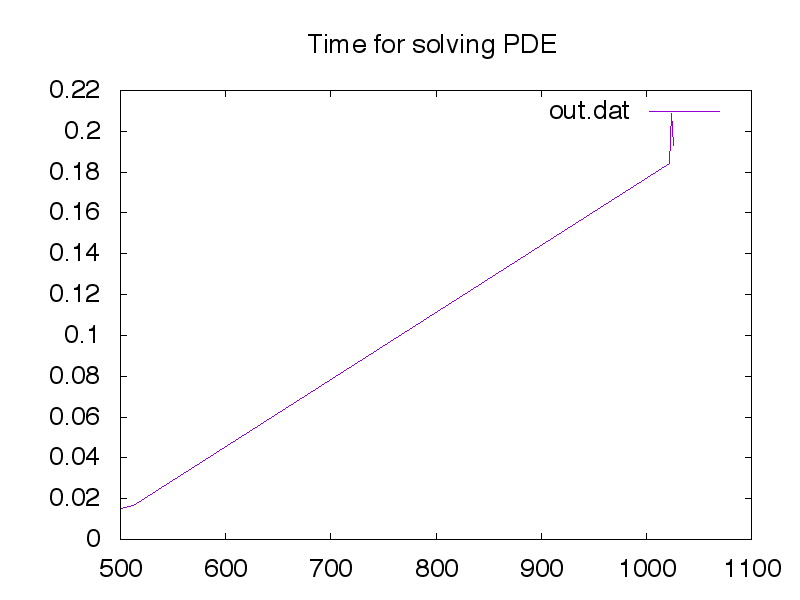
\includegraphics[width=90mm]{oldtime.png}
		\caption{Tempo para N\{x,y\} = \{500, 512\} no programa alterado para consumir menos memória
		\label{overflow}}
	\end{figure}
	
	O programa original foi implementado com a matriz A completa.
	Isto fez com que houvesse muito uso de memória, de modo que na achel não era possível executar discretizações grandes suficientes para o gráfico de tempo iniciado em 500.
	
	Fizemos uma alteração para reduzir o uso de memória, mas ainda assim só foi possível executar discretizações de até 512 separações em x e y.
	
	\subsection{Programa Otimizado}
	\subsubsection{Limite Superior da Discretização}

	\begin{align}
		T &\cong n_x + 1 = n_y + 1 \\
		|X| &= (n_x+1)\times(n_y+1)\times8 bytes \cong T^2\times8 bytes \\
		|B| &= (n_x+1)\times(n_y+1)\times8 bytes \cong T^2\times8 bytes \\
		|R| &= (n_x+1)\times(n_y+1)\times8 bytes \cong T^2\times8 bytes \\
		|X| + |B| + |R| &= 24000000000 \\
		3\times T^2\times8 &= 24000000000 \\
		T^2 &= 1000000000\\
		T &\cong 31622
	\end{align}

	A nova versão do programa aceita valores de até aproximadamente 31.622 para $n_y$ e $n_x$ numa máquina com 24GB de 	RAM e desconsiderando o uso de memória virtual e qualquer outro uso de memória que seja necessário.
	%Ou seja, pode computar até 54.756 de pontos.
	
	Apesar do programa original ser um desastre, o novo programa é razoável, mas mesmo assim uma bosta. Sabe porque? por causa da porra da alemanha chamada likwid! caralho.
	
	\subsubsection{Tempo de Execução}
	\begin{figure}[ht!]
		\centering
		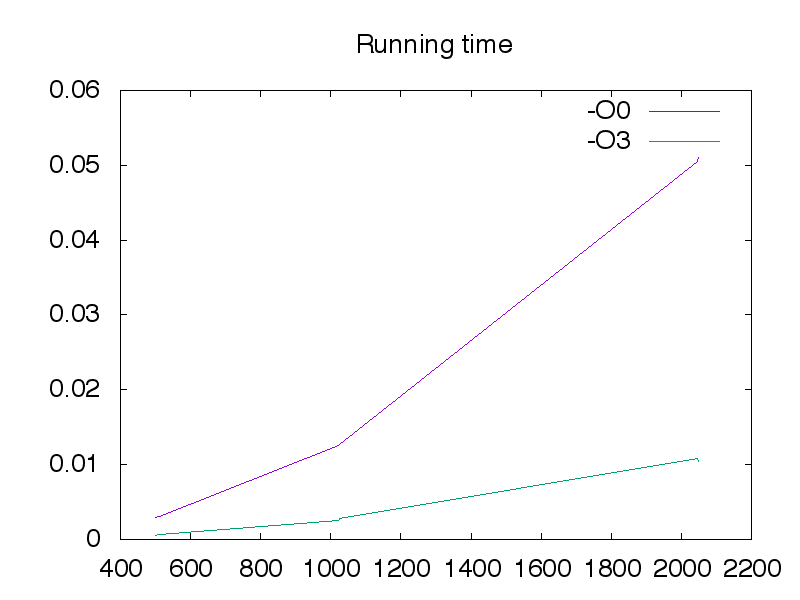
\includegraphics[width=90mm]{newtime.png}
		\caption{Tempo para N\{x,y\} = \{500, 512, 1022, 1024, 1026, 2046, 2048\} no novo programa
		\label{overflow}}
	\end{figure}
\newpage

% ------------------------------------------------------ %
\section{Análise de Funções}

	\subsection{Programa Original}
		\subsubsection{Método de Gauss-Seidel}
		\subsubsection{Cálculo do Resíduo}
	
	\subsection{Programa Otimizado}
		\subsubsection{Método de Gauss-Seidel}
		\subsubsection{Cálculo do Resíduo}

	\subsection{Análise dos Dados}

\newpage

% ------------------------------------------------------ %
\section{Otimização do Ponto de Interesse}

O ponto de interesse escolhido foi o cálculo do vetor $x$ no método de Gauss-Seidel.
Para isso, otimizações foram feitas nas estruturas de dados usadas durante o cálculo e na estrutura do laço em si.

	\subsection{Estrutura de dados}
	A estrutura de dados que mais sofreu alterações foi a matriz $A$.
	Na versão original do programa, $A$ tinha o tamanho de $((n_x+1)\times(n_y+1))^2$, representando a matriz inteira do método analítico de Gauss Seidel.
	
	Olhando para a matriz $A$, percebemos que grande parte das posições tinham valor $0$ e que os valores de interesse de cada linha estavam numa distância de $(n_y+1)$ da diagonal principal da matriz.
	Ou seja, os dados que estavam além desse intervalo eram sempre $0$ e poderiam ser ignorados.
	
	Além disso, percebemos que as posições ao redor da diagonal principal sempre seguiam o seguinte padrão:
	
	\begin{center}
		\texttt{$h_x$ 0 $h_y$ 1 $h_y$ 0 $h_x$}
	\end{center}
	
	Onde o elemento na diagonal principal é sempre $1$, $h_x$ e $h_y$ representam a dependência dos pontos adjacentes e, no exemplo acima, $n_y=2$.
	Sendo assim, podíamos ignorar as posições que sempre continham $1$ ou $0$, além de evitar a repetição de $h_x$ e $h_y$.
	
	Também foi possível ver que os valores de $h_x$ e $h_y$ permaneciam constantes em quase todas as linhas da matriz, exceto nas linhas em que não estavam presentes.
	As linhas que não continham $h_x$ e $h_y$ representavam os pontos das bordas da grade, que são calculadas separadamente.
	Logo, foi possível ver que uma matriz que simplesmente nos dizia se um determinado ponto é ou não uma borda era suficiente para fazer os cálculos de Gauss-Seidel, se salvássemos $h_x$ e $h_y$ em variáveis separadas.
	
	Portanto, a matriz $A$ passou a ter o tamanho de $(n_x+1)\times(n_y+1)$ e utiliza o tipo de dados \emph{short int}, pois apenas armazenamos $0$ quando o ponto é uma borda ou $1$ caso contrário.
	
	Após isso, percebemos que não havia necessidade de armazenar essas informações em um vetor de qualquer maneira.
	Assim, modificamos o laço do Gauss-Seidel para que percorra apenas as posições relevantes de $x$ e $B$ (que correspondem aos pontos que não são bordas).
	Dessa forma, é possível evitar condições durante o laço, pois os elementos de $x$ correspondentes a posições de borda serão $0$ e, na multiplicação, tornarão os valores a serem desconsiderados em $0$ também.
	
	Na versão nova do programa, então, não há qualquer representação para a matriz A, e essa parte do problema foi resolvida de forma algébrica.

	\subsection{Código}
	
	Na versão anterior do programa, o laço de Gauss-Seidel continha quatro desvios condicionais, um para cada borda.
	Nesta versão, não temos mais desvios porque, se o resultado de uma operação deve ser desconsiderado, essa operação resultará em $0$.
	
	Quatro operações são realizadas utilizando os valores de $h_x$ e $h_y$ e outras posições do vetor $x$ (que são $0$ se representa um ponto de borda).
	Na versão original do programa, as quatro operações eram armazenadas na variável \texttt{temp} utilizando o operador \texttt{+=}.
	Isso causava problemas no pipeline da execução, pois gerava uma dependência de dados onde todas as operações em ponto flutuante da linha anterior precisavam ser computadas antes do início dos cálculos da próxima.
	Agora, as quatro operações são salvas em variáveis separadas para permitir melhor uso do pipeline. 
	Essas quatro variáveis são então computadas após as quatro operações.
	
	Adicionalmente, utilizamos a técnica de \emph{loop unrolling} de passo 2 para melhorar ainda mais o desempenho do programa.
	Ao invés de quatro operações principais, cada iteração do laço agora faz oito operações.
	Experimentamos aumentar o passo do \emph{unroll} para 4, mas a diferença no tempo de execução foi irrisória e optamos por continuar utilizando passo 2 para manter a legibilidade do código.
	
	Todas otimizações foram replicadas no laço que calcula o resíduo do método de Gauss-Seidel e obtivemos melhoras semelhantes de desempenho.

\newpage

% ------------------------------------------------------ %
% Resultados %
\section{Resultados}

\subsection{Tempo}

\subsection{Memória}

\newpage

\end{document}